%---------------------------------- Large Language Models -------------------------------
\begin{frame}{Large Language Models}
\begin{columns}
      
    \begin{column}[t]{0.4\textwidth}
    \begin{block}{Summary}
    
        \begin{itemize}
            \item State-of-the-art of Natural Language Processing (NLP) problems
            \item Architecture : Transformers\footnote{Vaswani et al., « Attention is All you Need ».} block, mixed with classical layers (MLP, Conv)
            \item Huge size : Billions of parameters (1B to 405B for Llama 3)
            \item 2 phases of training : pre-training and \textbf{fine-tuning}
        \end{itemize}
            

    \end{block}
    \end{column}
        
    \begin{column}[t]{0.55\textwidth}
    \begin{block}{Self Attention }

        \begin{figure}
            \centering
            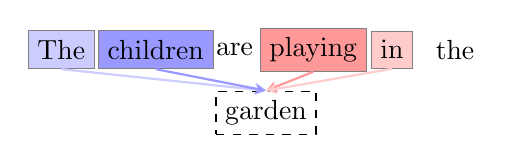
\begin{tikzpicture}[node distance=0.8cm]

    % Define block styles
    \tikzstyle{model} = [rectangle,rounded corners, minimum width=2cm, minimum height=1cm, text centered, draw=black, fill=blue!30]
    \tikzstyle{arrow} = [thick,->,>=stealth]
    
    % Define nodes
    \node (the) [fill=blue!20,rectangle,draw=black!50] {The};
    \node (children) [right of = the,fill=blue!40,rectangle,draw=black!50,xshift=0.4cm] {children};
    \node (are) [right of = children,xshift=0.2cm] {are};
    \node (playing) [right of = are,fill=red!40,rectangle,draw=black!50,xshift=0.2cm] {playing};
    \node (in) [right of = playing,fill=red!20,rectangle,draw=black!50,xshift=0.2cm] {in};
    \node (the2) [right of = in] {the};
    
    \node (garden) [below of = are, xshift=0.4cm,rectangle,dashed,draw=black] {garden};
    
    % Draw arrows
    \draw [arrow,draw=blue!20] (the.south) -- (garden.north);
    \draw [arrow,draw=blue!40] (children.south) -- (garden.north);
    \draw [arrow,draw=red!40] (playing.south) -- (garden.north);
    \draw [arrow,draw=red!20] (in.south) -- (garden.north);
    
    % Add a rectangle around the last four nodes
    \end{tikzpicture}
            \caption{Self Attention mecanism illustration}
        \end{figure}
    
        Self attention is the key of LLM, used to compute the context of each token.
    \end{block}  
    \end{column}
         
\end{columns}
\end{frame}

%---------------------------------- Fine-tuning Workflow -------------------------------

\begin{frame}{Fine-Tuning}

    Following a first phase of pre-training, Fine-tuning is used to correct behavior or add in-domain data to a model, with limited resources. 


    \begin{figure}
        \centering
        \resizebox{\textwidth}{!}{
            \begin{tikzpicture}[node distance=1.5cm]

% Define block styles
\tikzstyle{model} = [rectangle,rounded corners, minimum width=2cm, minimum height=1cm, text centered, draw=black, fill=blue!30]
\tikzstyle{data} = [rectangle, rounded corners, minimum width=2cm, minimum height=1cm,text centered, draw=black, fill=yellow!30]
\tikzstyle{action} = [rectangle, rounded corners, minimum width=2cm, minimum height=1cm,text centered, draw=black, fill=red!30]
\tikzstyle{arrow} = [thick,->,>=stealth]

% Define nodes
\node (model1) [model,align=center] {Model\\Random init};
\node (data1) [data, below of=model1,align=center]{Pre-Training \\ Data Corpus} ;
\node (pre-train)[action, right of=model1, xshift=1.5cm,yshift=-1cm]{Pre-Training};
\node (model2) [model, right of=pre-train, xshift = 1.5cm, yshift=1cm ]{Pre-Trained Model};
\node (data2) [data, below of= model2]{In-domain data};
\node (fine-tuning)[action, right of = model2, xshift = 1.5cm,yshift=-1cm]{Fine Tuning};
\node (model3) [model, right of=fine-tuning, xshift = 1.5cm,align=center ]{Fine-Tuned \\ model};


% Draw arrows
\draw [arrow] (data1) -- (pre-train);
\draw [arrow] (model1) -- (pre-train);
\draw [arrow] (pre-train) -- (model2);
\draw [arrow] (model2) -- (fine-tuning);
\draw [arrow] (data2) -- (fine-tuning);
\draw [arrow] (fine-tuning) -- (model3);

% Add a rectangle around the last four nodes
\node[draw, thick, dashed, rounded corners, fit=(model2) (fine-tuning) (model3) (data2), inner sep=0.3cm, label=above:{Fine-Tuning Framework}] {};
\end{tikzpicture}
        }
        \caption{Pre-training and Fine-tuning generic workflow}
    \end{figure}  
        

    
\end{frame}

%---------------------------------- Fine Tuning Frame -------------------------------
\begin{frame}{Parameters Efficient Fine-Tuning (PEFT)}
    Set of methods aims to reduce the computation cost of fine-tuning. 2 main approaches : \textit{Additive} and \textbf{reparametrization}.
    
    \begin{columns}  
  
        \begin{column}[t]{0.45\textwidth}
        \begin{block}{Reparametrization}
            Use lower-cost proxy as trainable weights, and merge at the end. e.g. : LoRA and derived methods
        \end{block}
        \end{column}
    
        \begin{column}[t]{0.45\textwidth}
        \begin{block}{Additive}
            Add part of the model, often linear layer, to train these.  One con is to add inference to generation.
            
        \end{block}
        \end{column}
      
    \end{columns}

    \begin{block}{Quantization}
        To reduce further the cost of computing during the training, quantization can also be used. This can be combined with either of precedent approaches. 
        
    \end{block}

\end{frame}



%---------------------------------- LoRA -------------------------------
\begin{frame}{Low Rank Adaptation (LoRA)}
    \begin{block}{Principle}
        Merging Fine-tuning layers with pre-trained ones can be written as $W = W_0 + \Delta W$, with $W_0$ the pre-trained weights and $\Delta W$ the fine-tuned ones. With LoRA, $W=W_0 + \frac{\alpha}{r} B.A$        
    \end{block}

    \begin{columns}
        \begin{column}[t]{0.45\textwidth}
        \begin{figure}
            \centering
            \resizebox{\textwidth}{!}{
                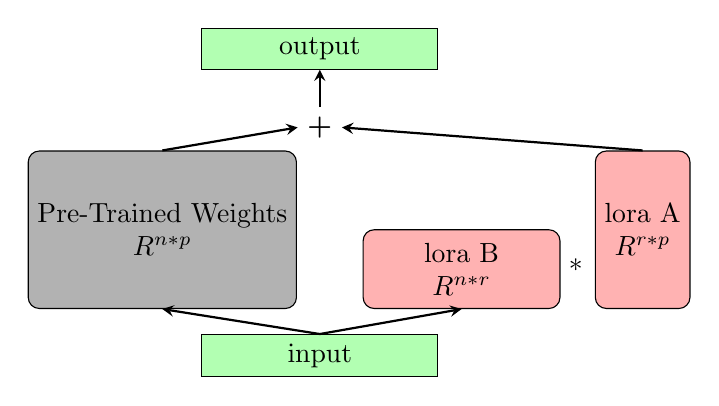
\begin{tikzpicture}[node distance=1.8cm]
    % Define block styles
    \tikzstyle{weights} = [rectangle,rounded corners, minimum width=2.5cm, minimum height=2cm, text centered, draw=black, fill=black!30]
    \tikzstyle{lora_a} = [rectangle,rounded corners, minimum width=1cm, minimum height=2cm, text centered, draw=black, fill=red!30]
    \tikzstyle{lora_b} = [rectangle,rounded corners, minimum width=2.5cm, minimum height=1cm, text centered, draw=black, fill=red!30]
    \tikzstyle{vector} = [rectangle, minimum width=3cm, minimum height=0.5cm, text centered, draw=black, fill=green!30]
    \tikzstyle{arrow} = [thick,->,>=stealth]
    
    % Define nodes
    \node (weights) [weights, align=center]{Pre-Trained Weights \\ $\mathbb{R}^{n*p}$};
    \node (lora_B) [lora_b, right of=weights,xshift=2cm,yshift=-0.5cm, align=center]{lora B\\ $\mathbb{R}^{n*r}$};
    \node (mul) [right of = lora_B,xshift=-0.35cm]{*};
    \node (lora_A) [lora_a, right of=lora_B,xshift=0.5cm,yshift=0.5cm, align=center]{lora A\\$\mathbb{R}^{r*p}$};
    \node (input) [vector,below of = weights, xshift = 2cm,yshift=+0.2cm]{input};
    \node (plus) [above of = weights, xshift = 2cm,yshift=-0.5cm]{\textbf{+}};
    \node (output) [vector,above of = plus,yshift=-0.8cm]{output};
    
    
    
    
    % Draw arrows
    \draw [arrow] (input.north) -- (weights.south);
    \draw [arrow] (input.north) -- (lora_B.south);
    \draw [arrow] (weights.north) -- (plus.west);
    \draw [arrow] (lora_A.north) -- (plus.east);
    \draw [arrow] (plus) -- (output);
    
    
    \end{tikzpicture}
            }
            \caption{LoRA Decomposition}
        \end{figure}
            
        \end{column}
        
        \begin{column}[t]{0.3\textwidth}
            \begin{block}{LoRA hyperparameters}
            \begin{itemize}
                \item rank $r$ : the common dimension between $A$ and $B$.
                \item alpha $\alpha$ : apply a weighting between fine-tuning and pre-trained weights
            \end{itemize}
                
            \end{block}
            
        \end{column}
    \end{columns}
    
\end{frame}

%---------------------------------- HPO -------------------------------
\begin{frame}{Hyperparameter Optimization (HPO)}

    \begin{columns}
         
        %%%%%%%%%%%%%%%%%%%%%%%%%% COLONNE DE GAUCHE %%%%%%%%%%%%%%
           \begin{column}{0.3\textwidth} 
           \begin{block}{Objectives}
            \begin{itemize}
                \item Better performance than manual tuning
                \item Ease popularization of the Fine Tuning
            \end{itemize}
            
           \end{block}
    
           \end{column}
               
        %%%%%%%%%%%%%%%%%%%%%%%%% COLONNE DE DROITE %%%%%%%%%%%%%%
           \begin{column}{0.7\textwidth}
            \begin{figure}
                \centering
                \resizebox{\textwidth}{!}{
                    \begin{tikzpicture}[node distance=2cm]

% Define block styles
\tikzstyle{startstop} = [rectangle, rounded corners, minimum width=3cm, minimum height=1cm,text centered, draw=black, fill=green!30]
\tikzstyle{io} = [trapezium, trapezium left angle=70, trapezium right angle=110, minimum width=3cm, minimum height=1cm, text centered, draw=black, fill=blue!30]
\tikzstyle{process} = [rectangle, minimum width=3cm, minimum height=1cm, text centered, draw=black, fill=blue!20]
\tikzstyle{decision} = [diamond, minimum width=3cm, minimum height=1cm, text centered, draw=black, fill=red!30]
\tikzstyle{arrow} = [thick,->,>=stealth]

% Nodes
\node (start) [startstop] {Training Data};
\node (preprocess) [process, below of=start] {Preprocessing};
\node (stop) [decision, below of=preprocess] {Stop?};
\node (hpo) [process, right of=stop, xshift=3cm] {Hyperparameter Optimization (HPO)};
\node (finalmodel) [startstop, below of=stop] {Final Model};
\node (validation) [startstop, above of=hpo] {Validation Data};

% Arrows
\draw [arrow] (start) -- (preprocess);
\draw [arrow] (preprocess) -- (stop);
\draw [arrow] (stop) -- node[anchor=south] {No} (preprocess);
\draw [arrow] (stop) -- node[anchor=south] {Yes} (finalmodel);
\draw [arrow] (finalmodel) -- (hpo);
\draw [arrow] (validation) -- (hpo);
\draw [arrow] (hpo) -- (finalmodel);
\end{tikzpicture}
                }
                \caption{HPO workflow}
           \end{figure}  
           \end{column}
                
       \end{columns}

\end{frame}

%---------------------------------- Review Summary -------------------------------
\begin{frame}{Related Works}
    \begin{figure}
        \resizebox{0.9\textwidth}{!}{
            \begin{tikzpicture}[node distance = 1.15cm]

\tikzstyle{field} = [rectangle,rounded corners, minimum width=2cm, minimum height=0.8cm, text centered, draw=black]
\tikzstyle{art} = [rectangle split, rectangle split parts = 2, minimum width=2cm, minimum height=0.8cm, text centered, draw=black, fill=blue!30]
\tikzstyle{arrow} = [thick, ->, >=stealth]


% base
\node (base)[field, fill = violet!30]{LLM and Optimization \cite{wu_evolutionary_2024}};

% lvl 1
\node (opt_llm)[field, below of = base, xshift = -3cm, fill = blue!30]{Optimization to LLM};

\node (llm_opt)[field, below of = base, xshift = 3cm, fill = purple!30]{LLM to Optimization};

% lvl 2
\node (autodnn)[field, below of = opt_llm, xshift = -0.5cm, fill=teal!30]{AutoDNN};
\node(prompt)[art,right of = autodnn, xshift = 2.5cm, fill = blue!20]{
    \textbf{Prompt Eng.}
    \nodepart{second} Art. \cite{guo_connecting_2024}
};
\node (gen_ea)[art, below of = llm_opt, fill = purple!20]{
    \textbf{Generate EA}
    \nodepart{second} Art. \cite{liu_large_2024}
};

% lvl 3
\node (hpo)[field, below of = autodnn, xshift = -1.5cm, fill = cyan!50]{HPO};
\node (nas)[field, right of = hpo, xshift = 3.5cm, fill = green!30]{NAS};

% lvl4 hpo

\node (hpo_ft)[art, below of = hpo, fill = cyan!35]{
    \textbf{Fine-Tuning}
    \nodepart{second} Art. \cite{tribes_hyperparameter_2024}
};
\node (hpo_pt)[art, left of = hpo_ft, xshift = -1cm, fill = cyan!20]{
    \textbf{Pre-training}
    \nodepart{second} -
};
\node (hpo_gen)[art, right of = hpo_ft,xshift = 1cm, fill = cyan!20]{
    \textbf{Generation}
    \nodepart{second} Art. \cite{wang_cost-effective_2023}
};
% lvl4 nas
\node (nas_scratch)[art, below of = nas, fill = green!20]{
    \textbf{From Scratch}
    \nodepart{second} Art. \cite{gao_autobert-zero_2022}
};
\node (nas_pruning)[art, right of = nas_scratch,xshift = 1cm, fill = green!20]{
    \textbf{Pruning}
    \nodepart{second} Art. \cite{klein_structural_2023}
};

% arrows
\draw[arrow] (base) -- (opt_llm);
\draw[arrow] (base) -- (llm_opt);

\draw[arrow] (opt_llm) -- (autodnn);
\draw[arrow] (opt_llm) -- (prompt);
\draw[arrow] (llm_opt) -- (gen_ea);

\draw[arrow] (autodnn) -- (hpo);
\draw[arrow] (autodnn) -- (nas);

\draw[arrow] (hpo) -- (hpo_pt);
\draw[arrow] (hpo) -- (hpo_ft);
\draw[arrow] (hpo) -- (hpo_gen);

\draw[arrow] (nas) -- (nas_scratch);
\draw[arrow] (nas) -- (nas_pruning);

% fitting box
\node (current)[draw,thick, dashed, rounded corners, 
    fit = (hpo)(hpo_ft), inner sep = 0.2cm,
    label = below :{Current work}]{};

\end{tikzpicture}
        }
        \caption{Summary of links between LLM and Optimization}
    \end{figure}
    
    
\end{frame}